\chapter{Navigation---Groupby/Attrby}
\lhead{Chapter 2. \emph{Navigation---Groupby/Attrby}} % this is for the header on each page - perhaps a shortened title

Groupby means "Group by Property", it groups search results into each property value. Attrby means "Group by Attribute", it groups search results according to each attribute value.
Such kinds of grouping is frequently used in search navigation for such vertical searchs as e-commerce,..,etc. 

\section{Index Structure}
\label{GroupIndex}

The index structure for both Groupby and Attrby search is based on a forward index, as shown in \ref{fig:group_index}. 
In order to save the memory cost, the property value strings are mapped to ids. For each docid, we need to store an array of value ids, as the number of value ids might be 
different for each docid. The group index structure consists of two tables, one is \textbf{index table}, the other is \textbf{value id table}.
The \textbf{index table} stores index (or value id) for each docid. If this doc has only one value id, then it stores the value id direcly.

While if it has multiple value ids, then it stores the index in the \textbf{value id table}.In order to differentiate these two cases, we use the most significant bit.
That is, bit 0 for the case of single value id, and bit 1 for the other case.  In the \textbf{value id table}, the 1st entry is the number of value ids.
The following entries are each value id for the doc.

\begin{figure}[htp]
\centering
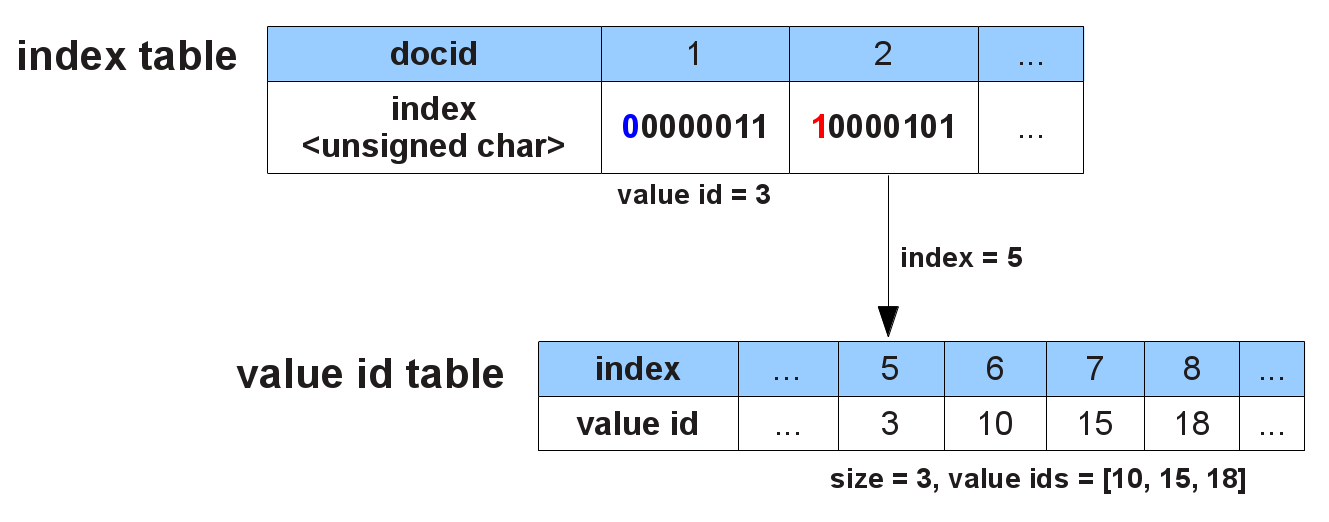
\includegraphics[width=0.8\textwidth]{Figures/group_index.png}
\caption{Group Index Example}\label{fig:group_index}
\end{figure}

In the example of figure \ref{fig:group_index}, the index type is parameterized as unsigned char. The docid 1 has only one value id (3), and the docid 2 has three value ids 
(10, 15 and 18).


\section{SCD Format}

The Groupby search requires corresponding property type to be string, it supports hierarchical values. Below is its SCD format:
\begin{lstlisting}
<PropertyName>A>B>C,D>E>F...
\end{lstlisting}

\begin{itemize}
\item The \verb!PropertyName! is the property name which needs group results;
\item The property could contain multiple values, each separated by comma \verb!,! or semicolon \verb!;!
\item If the value has parent value, you need to specify the whole path from root to leaf node, each separated by symbol \verb!>!
\item If one attribute name contains multiple values, such as A, B and C, each value is separated by the vertical line \verb!|!, for example, \verb!name:A|B|C!
\item In property values, if there is any embedded character of comma \verb!,!, semicolon \verb!;!, symbol \verb!>! or double-quote \verb!"!,
the whole value must be surrounded by double-quotes.
And the embedded double-quotes must each be represented by a pair of consecutive double quotes.
For example, if the property value contains values on three levels. The root value is John, Mark. The 2nd level value is 1+1>2. The 3rd level value is "Mary".
Then you need to specify it as \verb!"John, Mark">"1+1>2">"""Mary"""! in SCD file

Please note that all of the above punctuations and symbols are half width.

\end{itemize}

The Attrby search also requires the attribute property type to be string with such kinds of format:
\begin{lstlisting}
<PropertyName>name:value,name:value...
\end{lstlisting}

\begin{itemize}
\item The \verb!PropertyName! is the property name which contains pairs of attribute name and value.

\item Each pair of attribute name and value is separated by the comma \verb!,!

\item Attribute name and value are separated by the colon \verb!:!

\item If one attribute name contains multiple values, such as A, B and C, each value is separated by the vertical line \verb!|!, for example, \verb!name:A|B|C!

\item In attribute name or value, if there is any embedded character of above delimiters \verb!,:|! or double-quote \verb!"!, the whole attribute name or value must be surrounded by double-quotes.
And the embedded double-quotes must each be represented by a pair of consecutive double quotes \verb!""!.
For example, if the attribute name or value is \verb!John, Mark: "Mary" | Tom!, you need to specify it as \verb!"John, Mark: ""Mary"" | Tom"! in SCD file.

Please note that all of the above punctuations \verb!,:|"! are half width.

\end{itemize}


\section{Configuration}
\subsection{Groupby Search}
\begin{itemize}
\item In collection config file, such as \verb!config/example.xml! in sf1r-engine, for the property in \verb!DocumentSchema!,
if you need group results on this property (the property type must be string, int, float or datetime),
you have to configure it in \verb!MiningBundle/Schema/Group!.

\item If the property type is int or float, you also need to configure it as filter property in \verb!IndexBundle!.

\item For the property type of int and float, it's unnecessary to build group index data.

\item While for the property type of string and datetime, it would build group index data when each time SCD is indexed.
Normally, it starts from the last doc id when last time group index data is built.

\item If the string property is configured as \verb!<IndexBundle><Schema><Indexing ... rtype="y"/>!,
then for this RType string property, it would rebuild its whole group index data when each time SCD is indexed.

\item For other properties, if you want to rebuild the whole group index data when each time SCD is indexed,
you need to configure the "rebuild" attribute to "y". For example, \verb!<Group><Property name="Category" rebuild="y"/>!.

\end{itemize}

For example:

\begin{lstlisting}
<DocumentSchema>
  ...
  <Property name="Category" type="string" />
  <Property name="Price" type="float" />
  <Property name="PlayTime" type="datetime" />
</DocumentSchema>

<IndexBundle>
  <Schema>
    <Property name="Price">
      <Indexing filter="yes" multivalue="no" doclen="yes" tokenizer="" rankweight="0.1" />
    </Property>
    ...
  </Schema>
</IndexBundle>

<MiningBundle>
  <Schema>
    ...
    <Group>
      <Property name="Category" />
      <Property name="Price" />
      <Property name="PlayTime" />
    </Group>
  </Schema>
</MiningBundle>
\end{lstlisting}

\subsection{Attrby Search}
In collection config file, such as "config/example.xml" in sf1r-engine, for the property which contains attribute names and values,
you have to add it in \textbf{MiningBundle/Schema/Attr}. Please note that at most one property is allowed in \textbf{Attr} configuration.

If you want to exclude some attribute names, you need to configure them into \textbf{Exclude}.

For example:

\begin{lstlisting}
<DocumentSchema>
  ...
  <Property name="Attribute" type="string" />
</DocumentSchema>
...
<MiningBundle>
  <Schema>
    ...
    <Attr>
      <Property name="Attribute" />
      <Exclude name="ISBN" />
    </Attr>
  </Schema>
</MiningBundle>
\end{lstlisting}

